\documentclass{standalone}
\usepackage{tikz}
\usetikzlibrary{patterns, positioning}


\begin{document}
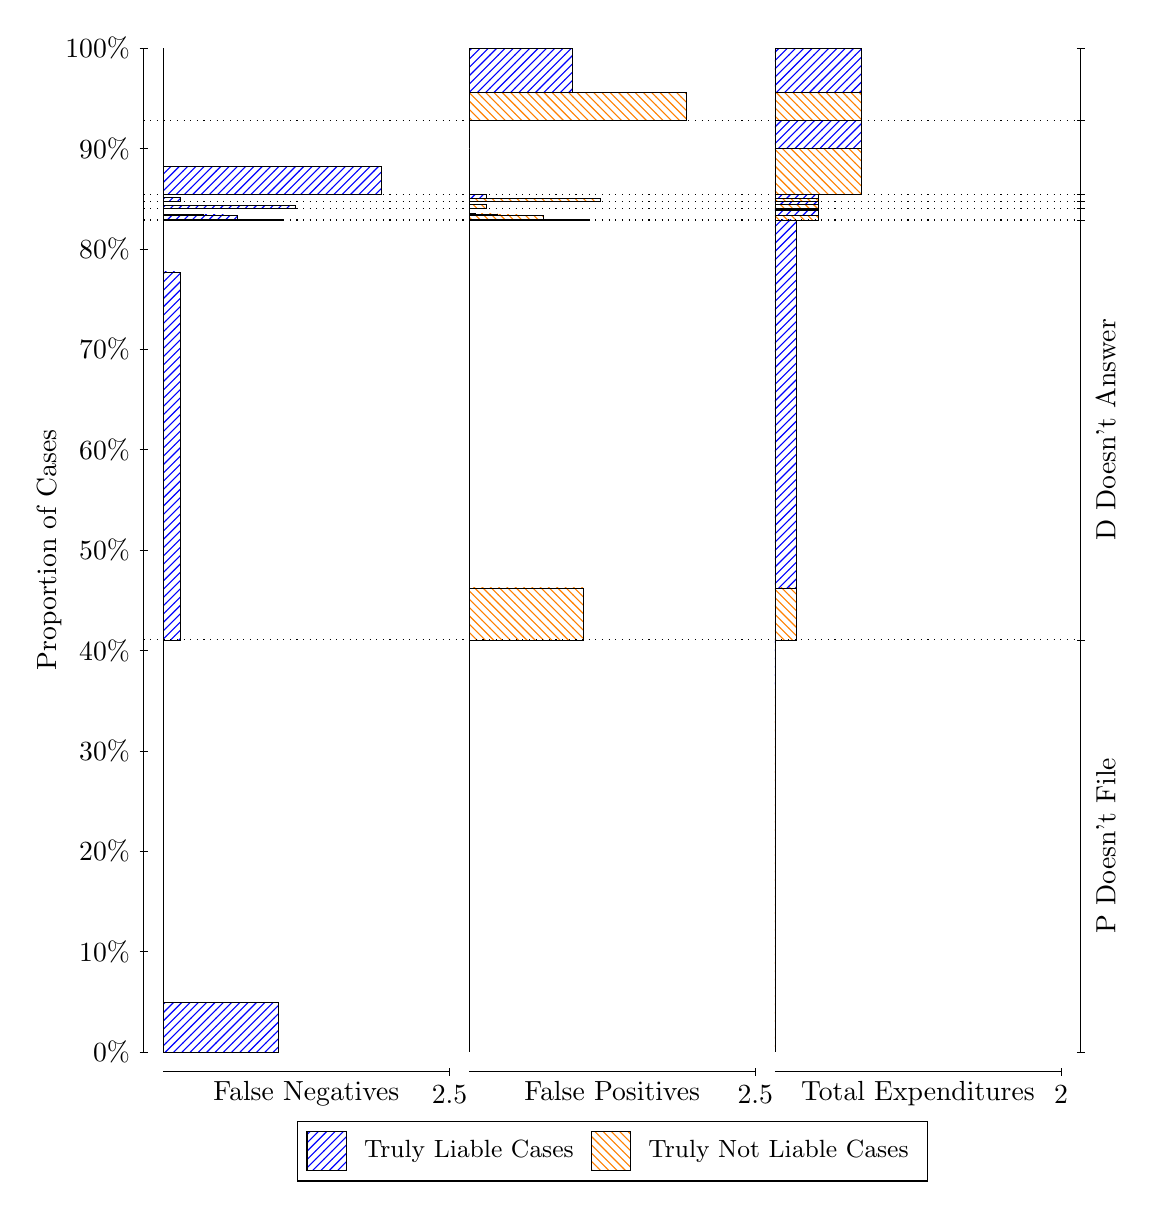
\begin{tikzpicture}
\draw[black, very thin] (1.5,1.75) -- (1.5,14.5);
\node[rotate=90, text=black, anchor=center] at (0.3, 8.125) {Proportion of Cases};
\draw[black, very thin] (1.45,1.75) -- (1.55,1.75);
\node[text=black, anchor=east] at (1.45, 1.75) {0\%};
\draw[black, very thin] (1.45,3.025) -- (1.55,3.025);
\node[text=black, anchor=east] at (1.45, 3.025) {10\%};
\draw[black, very thin] (1.45,4.3) -- (1.55,4.3);
\node[text=black, anchor=east] at (1.45, 4.3) {20\%};
\draw[black, very thin] (1.45,5.575) -- (1.55,5.575);
\node[text=black, anchor=east] at (1.45, 5.575) {30\%};
\draw[black, very thin] (1.45,6.85) -- (1.55,6.85);
\node[text=black, anchor=east] at (1.45, 6.85) {40\%};
\draw[black, very thin] (1.45,8.125) -- (1.55,8.125);
\node[text=black, anchor=east] at (1.45, 8.125) {50\%};
\draw[black, very thin] (1.45,9.4) -- (1.55,9.4);
\node[text=black, anchor=east] at (1.45, 9.4) {60\%};
\draw[black, very thin] (1.45,10.675) -- (1.55,10.675);
\node[text=black, anchor=east] at (1.45, 10.675) {70\%};
\draw[black, very thin] (1.45,11.95) -- (1.55,11.95);
\node[text=black, anchor=east] at (1.45, 11.95) {80\%};
\draw[black, very thin] (1.45,13.225) -- (1.55,13.225);
\node[text=black, anchor=east] at (1.45, 13.225) {90\%};
\draw[black, very thin] (1.45,14.5) -- (1.55,14.5);
\node[text=black, anchor=east] at (1.45, 14.5) {100\%};

\draw[black, very thin] (13.4,1.75) -- (13.4,14.5);
\draw[black, very thin] (13.35,1.75) -- (13.45,1.75);
\node[anchor=west] at (13.35, 1.75) {};
\draw[black, very thin] (13.35,6.9846) -- (13.45,6.9846);
\node[anchor=west] at (13.35, 6.9846) {};
\draw[black, very thin] (13.35,12.316) -- (13.45,12.316);
\node[anchor=west] at (13.35, 12.316) {};
\draw[black, very thin] (13.35,12.464) -- (13.45,12.464);
\node[anchor=west] at (13.35, 12.464) {};
\draw[black, very thin] (13.35,12.556) -- (13.45,12.556);
\node[anchor=west] at (13.35, 12.556) {};
\draw[black, very thin] (13.35,12.639) -- (13.45,12.639);
\node[anchor=west] at (13.35, 12.639) {};
\draw[black, very thin] (13.35,13.584) -- (13.45,13.584);
\node[anchor=west] at (13.35, 13.584) {};
\draw[black, very thin] (13.35,14.5) -- (13.45,14.5);
\node[anchor=west] at (13.35, 14.5) {};

\draw[black, very thin, pattern color=blue, pattern=north east lines] (1.75,1.75) rectangle (3.2033,2.378);
\draw[black, very thin, pattern color=orange, pattern=north west lines] (1.75,2.378) rectangle (1.75,6.9846);
\draw[black, very thin, pattern color=blue, pattern=north east lines] (1.75,6.9846) rectangle (1.968,11.656);
\draw[black, very thin, pattern color=orange, pattern=north west lines] (1.75,11.656) rectangle (1.75,12.316);
\draw[black, very thin, pattern color=blue, pattern=north east lines] (1.75,12.316) rectangle (3.276,12.322);
\draw[black, very thin, pattern color=blue, pattern=north east lines] (1.75,12.322) rectangle (3.1307,12.322);
\draw[black, very thin, pattern color=blue, pattern=north east lines] (1.75,12.322) rectangle (2.9853,12.324);
\draw[black, very thin, pattern color=blue, pattern=north east lines] (1.75,12.324) rectangle (2.84,12.325);
\draw[black, very thin, pattern color=blue, pattern=north east lines] (1.75,12.325) rectangle (2.6947,12.379);
\draw[black, very thin, pattern color=blue, pattern=north east lines] (1.75,12.379) rectangle (2.5493,12.38);
\draw[black, very thin, pattern color=blue, pattern=north east lines] (1.75,12.38) rectangle (2.404,12.382);
\draw[black, very thin, pattern color=blue, pattern=north east lines] (1.75,12.382) rectangle (2.2587,12.383);
\draw[black, very thin, pattern color=blue, pattern=north east lines] (1.75,12.383) rectangle (2.1133,12.386);
\draw[black, very thin, pattern color=orange, pattern=north west lines] (1.75,12.386) rectangle (1.75,12.464);
\draw[black, very thin, pattern color=blue, pattern=north east lines] (1.75,12.464) rectangle (3.4213,12.501);
\draw[black, very thin, pattern color=orange, pattern=north west lines] (1.75,12.501) rectangle (1.75,12.556);
\draw[black, very thin, pattern color=blue, pattern=north east lines] (1.75,12.556) rectangle (1.968,12.604);
\draw[black, very thin, pattern color=orange, pattern=north west lines] (1.75,12.604) rectangle (1.75,12.639);
\draw[black, very thin, pattern color=blue, pattern=north east lines] (1.75,12.639) rectangle (4.5113,12.999);
\draw[black, very thin, pattern color=orange, pattern=north west lines] (1.75,12.999) rectangle (1.75,13.584);
\draw[black, very thin, pattern color=orange, pattern=north west lines] (1.75,13.584) rectangle (1.75,13.939);
\draw[black, very thin, pattern color=blue, pattern=north east lines] (1.75,13.939) rectangle (1.75,14.5);
\draw[black, very thin, pattern color=orange, pattern=north west lines] (5.6333,1.75) rectangle (5.6333,6.3566);
\draw[black, very thin, pattern color=blue, pattern=north east lines] (5.6333,6.3566) rectangle (5.6333,6.9846);
\draw[black, very thin, pattern color=orange, pattern=north west lines] (5.6333,6.9846) rectangle (7.0867,7.6449);
\draw[black, very thin, pattern color=blue, pattern=north east lines] (5.6333,7.6449) rectangle (5.6333,12.316);
\draw[black, very thin, pattern color=orange, pattern=north west lines] (5.6333,12.316) rectangle (7.1593,12.319);
\draw[black, very thin, pattern color=orange, pattern=north west lines] (5.6333,12.319) rectangle (7.014,12.32);
\draw[black, very thin, pattern color=orange, pattern=north west lines] (5.6333,12.32) rectangle (6.8687,12.321);
\draw[black, very thin, pattern color=orange, pattern=north west lines] (5.6333,12.321) rectangle (6.7233,12.322);
\draw[black, very thin, pattern color=orange, pattern=north west lines] (5.6333,12.322) rectangle (6.578,12.376);
\draw[black, very thin, pattern color=orange, pattern=north west lines] (5.6333,12.376) rectangle (6.4327,12.378);
\draw[black, very thin, pattern color=orange, pattern=north west lines] (5.6333,12.378) rectangle (6.4327,12.378);
\draw[black, very thin, pattern color=orange, pattern=north west lines] (5.6333,12.378) rectangle (6.2873,12.38);
\draw[black, very thin, pattern color=orange, pattern=north west lines] (5.6333,12.38) rectangle (6.142,12.381);
\draw[black, very thin, pattern color=orange, pattern=north west lines] (5.6333,12.381) rectangle (5.9967,12.394);
\draw[black, very thin, pattern color=blue, pattern=north east lines] (5.6333,12.394) rectangle (5.706,12.398);
\draw[black, very thin, pattern color=blue, pattern=north east lines] (5.6333,12.398) rectangle (5.6333,12.464);
\draw[black, very thin, pattern color=orange, pattern=north west lines] (5.6333,12.464) rectangle (5.8513,12.519);
\draw[black, very thin, pattern color=blue, pattern=north east lines] (5.6333,12.519) rectangle (5.6333,12.556);
\draw[black, very thin, pattern color=orange, pattern=north west lines] (5.6333,12.556) rectangle (7.3047,12.591);
\draw[black, very thin, pattern color=blue, pattern=north east lines] (5.6333,12.591) rectangle (5.8513,12.639);
\draw[black, very thin, pattern color=orange, pattern=north west lines] (5.6333,12.639) rectangle (5.6333,13.225);
\draw[black, very thin, pattern color=blue, pattern=north east lines] (5.6333,13.225) rectangle (5.6333,13.584);
\draw[black, very thin, pattern color=orange, pattern=north west lines] (5.6333,13.584) rectangle (8.3947,13.939);
\draw[black, very thin, pattern color=blue, pattern=north east lines] (5.6333,13.939) rectangle (6.9413,14.5);
\draw[black, very thin, pattern color=orange, pattern=north west lines] (9.5167,1.75) rectangle (9.5167,6.3566);
\draw[black, very thin, pattern color=blue, pattern=north east lines] (9.5167,6.3566) rectangle (9.5167,6.9846);
\draw[black, very thin, pattern color=orange, pattern=north west lines] (9.5167,6.9846) rectangle (9.7892,7.6449);
\draw[black, very thin, pattern color=blue, pattern=north east lines] (9.5167,7.6449) rectangle (9.7892,12.316);
\draw[black, very thin, pattern color=orange, pattern=north west lines] (9.5167,12.316) rectangle (10.062,12.378);
\draw[black, very thin, pattern color=blue, pattern=north east lines] (9.5167,12.378) rectangle (10.062,12.44);
\draw[black, very thin, pattern color=orange, pattern=north west lines] (9.5167,12.44) rectangle (10.062,12.454);
\draw[black, very thin, pattern color=blue, pattern=north east lines] (9.5167,12.454) rectangle (10.062,12.459);
\draw[black, very thin, pattern color=orange, pattern=north west lines] (9.5167,12.459) rectangle (10.062,12.462);
\draw[black, very thin, pattern color=blue, pattern=north east lines] (9.5167,12.462) rectangle (10.062,12.464);
\draw[black, very thin, pattern color=orange, pattern=north west lines] (9.5167,12.464) rectangle (10.062,12.519);
\draw[black, very thin, pattern color=blue, pattern=north east lines] (9.5167,12.519) rectangle (10.062,12.556);
\draw[black, very thin, pattern color=orange, pattern=north west lines] (9.5167,12.556) rectangle (10.062,12.591);
\draw[black, very thin, pattern color=blue, pattern=north east lines] (9.5167,12.591) rectangle (10.062,12.639);
\draw[black, very thin, pattern color=orange, pattern=north west lines] (9.5167,12.639) rectangle (10.607,13.225);
\draw[black, very thin, pattern color=blue, pattern=north east lines] (9.5167,13.225) rectangle (10.607,13.584);
\draw[black, very thin, pattern color=orange, pattern=north west lines] (9.5167,13.584) rectangle (10.607,13.939);
\draw[black, very thin, pattern color=blue, pattern=north east lines] (9.5167,13.939) rectangle (10.607,14.5);
\draw[black, dotted] (1.5,6.9846) -- (13.4,6.9846);
\draw[black, dotted] (1.5,12.316) -- (13.4,12.316);
\draw[black, dotted] (1.5,12.464) -- (13.4,12.464);
\draw[black, dotted] (1.5,12.556) -- (13.4,12.556);
\draw[black, dotted] (1.5,12.639) -- (13.4,12.639);
\draw[black, dotted] (1.5,13.584) -- (13.4,13.584);
\draw[black, very thin] (1.75,1.5) -- (5.3833,1.5);
\node[text=black, anchor=north] at (3.5667, 1.5) {False Negatives};
\draw[black, very thin] (5.3833,1.45) -- (5.3833,1.55);
\node[text=black, anchor=north] at (5.3833, 1.45) {2.5};

\draw[black, very thin] (5.6333,1.5) -- (9.2667,1.5);
\node[text=black, anchor=north] at (7.45, 1.5) {False Positives};
\draw[black, very thin] (9.2667,1.45) -- (9.2667,1.55);
\node[text=black, anchor=north] at (9.2667, 1.45) {2.5};

\draw[black, very thin] (9.5167,1.5) -- (13.15,1.5);
\node[text=black, anchor=north] at (11.333, 1.5) {Total Expenditures};
\draw[black, very thin] (13.15,1.45) -- (13.15,1.55);
\node[text=black, anchor=north] at (13.15, 1.45) {2};

\node[text=black, centered, rotate=90] at (13.72, 4.3673) {P Doesn't File};
\node[text=black, centered, rotate=90] at (13.72, 9.6505) {D Doesn't Answer};






\draw (7.449999999999999,1.5) node[draw=none] (baseCoordinate) {};
\begin{scope}[align=center]
        \matrix[scale=0.5, draw=black, below=0.5cm of baseCoordinate, nodes={draw}, column sep=0.1cm]{
            \node[rectangle, draw, minimum width=0.5cm, minimum height=0.5cm, pattern color=blue, pattern=north east lines] {}; &
            \node[draw=none, font=\small, text=black] (B) {Truly Liable Cases}; &
            \node[rectangle, draw, minimum width=0.5cm, minimum height=0.5cm, pattern color=orange, pattern=north west lines] {}; &
            \node[draw=none, font=\small, text=black] (B) {Truly Not Liable Cases}; \\
            };
\end{scope}

\end{tikzpicture}
\end{document}